\documentclass[aspectratio=169, 10pt]{beamer}
\usetheme{metropolis}
% \usefonttheme{professionalfonts}

\usepackage[english]{babel}
\usepackage[style=authortitle,backend=biber]{biblatex}
\usepackage[utf8]{inputenc}
\usepackage{algorithmic}
\usepackage{amsfonts}
\usepackage{amsmath}
\usepackage{amssymb}
\usepackage{array}
\usepackage{booktabs}
\usepackage{caption}
\usepackage{colortbl}
\usepackage{csquotes}
\usepackage{graphicx}
\usepackage{heuristica}
\usepackage{hyperref}
\usepackage{mathptmx}
\usepackage{multirow}
\usepackage{pgfplots}
\usepackage{siunitx}
\usepackage{subcaption}
\usepackage{svg}
\usepackage{tabularx}
\usepackage{textcomp}
\usepackage{xcolor}
\usepackage{bm}

\addbibresource{references.bib}

\usetikzlibrary{calc}

% \pgfplotsset{compat=1.17}
\usepgfplotslibrary{statistics}

\definecolor{uniblue}{HTML}{00467f}
\definecolor{uniblueDark}{HTML}{002052}
\definecolor{uniblueLight}{HTML}{4671af}
\definecolor{blueGrey}{HTML}{cfd8dc}
\definecolor{red800Dark}{HTML}{8e0000}
\definecolor{green800Dark}{HTML}{005005}

\setbeamercolor{background canvas}{bg=white}
% \setbeamertemplate{frame footer}{\insertshortauthor}
\setbeamerfont{page number in head/foot}{size=\tiny}
% \setbeamercolor{footline}{fg=white, bg=uniblue}
\setbeamercolor{footline}{fg=uniblue}
\setbeamercolor{title}{fg=uniblueDark, bg=white}
\setbeamercolor{frametitle}{fg=white, bg=uniblue}
\setbeamercolor{progress bar}{fg=uniblueLight, bg=white}
\setbeamercolor{block title}{use=structure,fg=white,bg=uniblue}
\setbeamercolor{block body}{use=structure,fg=black,bg=blueGrey}
\setbeamercolor{block title alerted}{fg=white,bg=red800Dark}
\setbeamercolor*{block title example}{fg=white, bg=green800Dark}
\setbeamercolor{alerted text}{fg=red800Dark}
\setbeamercolor{footnote}{fg=black}
\setbeamertemplate{frametitle continuation}[from second]
\setbeamercolor*{bibliography entry title}{fg=black}
\setbeamercolor*{bibliography entry author}{fg=black}
\setbeamercolor*{bibliography entry location}{fg=black}
\setbeamercolor*{bibliography entry note}{fg=black}
% \setbeamertemplate{bibliography item}{}

\setbeamerfont{author}{size=\normalsize}
\setbeamerfont{institute}{size=\small}
\setbeamerfont{date}{size=\normalsize}

\newcommand{\vect}{\mathbf}

\DeclareMathOperator*{\argmax}{argmax}

\hypersetup{
    % colorlinks=false,
    colorlinks=true,
    linkcolor=blue,
    filecolor=blue,
    urlcolor=blue,
}

\title{COMPSCI 762 Tutorial 9}
% \subtitle{Tutorial on Bayesian Networks, kNN, SVM, MDP and Q-Learning}
\subtitle{Tutorial on Unsupervised Learning}
\author{Luke Chang}
\institute{The University of Auckland}
\date{May 2021}


\begin{document}

\frame{\titlepage}

% %-------------------------------------------------------------------------------
% \begin{frame}
%     \frametitle{Topics}

%     \tableofcontents
        
% \end{frame}

%-------------------------------------------------------------------------------
% \section{Cluster Analysis}
\begin{frame}
\frametitle{Unsupervised Learning - Cluster Analysis}

\begin{itemize}
    \item Cluster analysis is an unsupervised learning task.
    \item The task of clustering is to partition a set of objects such that objects in the same group are more similar to each other than those in other groups.
    \item Evaluation metrics: 
    \item \begin{itemize}
        \item \textit{Sum of Squared Error} (SSE)
        \item \textit{Sum of Squared Between}(SSB)
    \end{itemize}
    \item Algorithms we will cover: 
        \begin{itemize}
            \item K-means
            \item Hierarchical clustering
            \item DBSCAN: Density-based clustering
        \end{itemize}
\end{itemize}

\end{frame}

%-------------------------------------------------------------------------------
\begin{frame}
    \frametitle{K-means}
    
    \begin{itemize}
        \item Partition the data into clusters
        \item Hyperparameter: the number of clusters, $K$
        \item Each cluster is associated with a centroid
        \item Each point is assigned to the cluster with the closest centroid
        \item Iterative method: Update centroids in each iteration, converge until the centroids don't change
    \end{itemize}
    
    Limitations:
    \begin{itemize}
        \item When clusters have:
            \begin{itemize}
                \item Different sizes
                \item Different densities
                \item Non-globular shapes (hypersphere)
            \end{itemize}
        \item When data contains outliers
    \end{itemize}
\end{frame}

%-------------------------------------------------------------------------------
\begin{frame}
    \frametitle{K-means Pseudocode}
    
    \hrulefill \par

    \begin{tabbing}
        Select $K$ points as the initial centroids \\
        \textbf{repeat:}\= \\
        \> \textbf{For} \= each point: \\
        \> \> Assign the point to the closest centroid \\
        \> \textbf{For} \= $i \in \{1, \ldots, K\}$ : \\
        \> \> Update the $i$ centroid \\
        \textbf{until} The centroids (or points) don't change
    \end{tabbing}

    \hrulefill \par
    
\end{frame}

%-------------------------------------------------------------------------------
\begin{frame}
    \frametitle{Evaluation Metric: Sum of Squared Error (SSE)}
    
    \begin{itemize}
        \item No true labels are available in the unsupervised learning
        \item Use sum of the squared errors to evaluate the performance
    \end{itemize}

    \[
        \text{SSE} = \sum^{K}_{i=1} \sum_{x \in C_i} \text{dist}^2(m_i, x)
    \]

    \begin{itemize}
        \item SSE highly depends on \textbf{K} and the \textbf{initial centroids}
        \item Depends on the initial $K$-centroids, the K-means clusters with same the $K$ value may not have the same SSE
    \end{itemize}
    
\end{frame}

%-------------------------------------------------------------------------------
\begin{frame}
    \frametitle{Solve the Initial Centroids Problem}
    
    \textbf{Problem:} Stuck in the local minimal 

    \begin{example}
        \href{https://scikit-learn.org/stable/auto\_examples/cluster/plot\_kmeans\_assumptions.html}{Demonstration of k-means assumptions from \textit{sklearn}}
    \end{example}

    \textbf{Solution:}
    \begin{itemize}
        \item Multiple runs
        \item Use hierarchical clustering to determine the initial centroids
        \item Define more than $K$ initial centroids and then select among these initial centroids
        \item Postprocessing:
            \begin{itemize}
                \item Remove empty clusters and small cluster
                \item Split ``loose'' clusters -- High SSE
                \item Merge clusters when they are ``close'' -- Low SSE
                \item Apply these steps multiple times and use the pruned centroids as new initial centroids
            \end{itemize}
        \item Improved k-means algorithms: Bisecting K-means, Mini Batch K-Means
    \end{itemize}
 
\end{frame}

%-------------------------------------------------------------------------------
\begin{frame}[t]
    \frametitle{Review Question 1: K-means}
    \small
    
    The distance matrix based on the Euclidean distance is given below:
    
    \begin{figure}
        \centering
        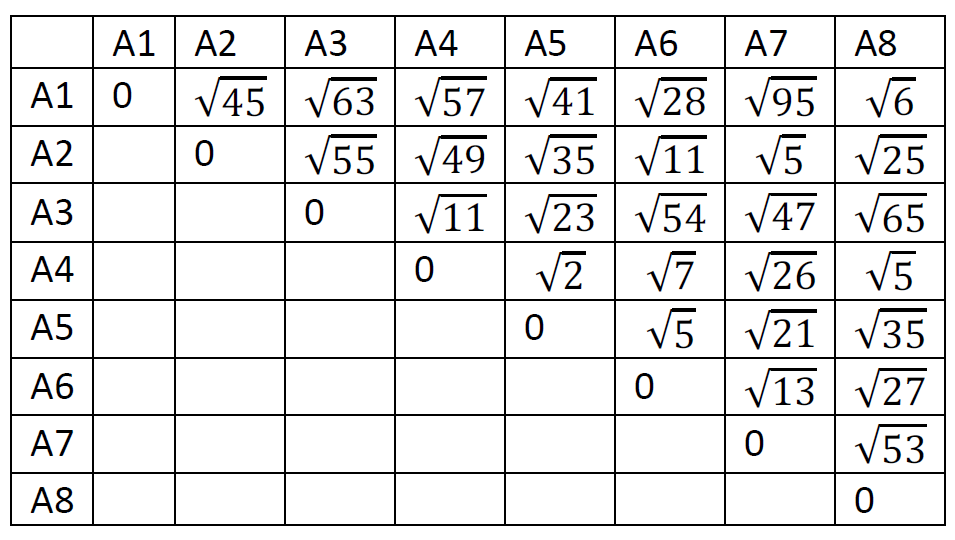
\includegraphics[width=0.5\textwidth]{../imgs/k-mean_review_q1.png}
    \end{figure}

    Suppose that the initial seeds (centers of each cluster) are \textbf{A1}, \textbf{A4} and \textbf{A7}. 
    Run the k-means algorithm for 1 epoch only. At the end of this epoch show:
    \begin{itemize}
        \item The new clusters (i.e. the examples belonging to each cluster)
        \item The centers of the new clusters
    \end{itemize}

\end{frame}

%-------------------------------------------------------------------------------
\begin{frame}[t]
    \frametitle{Review Question 1: K-means}
    \small
    
    \begin{columns}[]
        \begin{column}{0.5\textwidth} 
            \textbf{C1} is centred at \textbf{A1}, \textbf{C2} is centred at \textbf{A4}, and \textbf{C3} is centred at \textbf{A7}.\\
            For each point:\\
            \begin{itemize}
                \item $\textbf{A1} \rightarrow \textbf{C1}$
                \begin{table}[]
                    \scriptsize
                    \begin{tabular}{ccc}
                    Item & Centroid & Dist \\ \hline
                    A2   & A1       & $\sqrt{45}$ \\
                    A2   & A4       & $\sqrt{49}$ \\
                    A2   & A7       & $\sqrt{5}$
                    \end{tabular}
                \end{table}
                \item $\textbf{A2} \rightarrow \textbf{C3}$
                \begin{table}[]
                    \scriptsize
                    \begin{tabular}{ccc}
                    Item & Centroid & Dist \\ \hline
                    A3   & A1       & $\sqrt{63}$ \\
                    A3   & A4       & $\sqrt{11}$ \\
                    A3   & A7       & $\sqrt{47}$
                    \end{tabular}
                \end{table}
                \item $\textbf{A3} \rightarrow \textbf{C2}$
                \item $\textbf{A4} \rightarrow \textbf{C2}$
            \end{itemize}
        \end{column}
        \begin{column}{0.5\textwidth} 
            \begin{table}[]
                \scriptsize
                \begin{tabular}{ccc}
                Item & Centroid & Dist \\ \hline
                A5   & A1       & $\sqrt{41}$ \\
                A5   & A4       & $\sqrt{2}$ \\
                A5   & A7       & $\sqrt{21}$
                \end{tabular}
            \end{table}
            \begin{itemize}
                \item $\textbf{A5} \rightarrow \textbf{C2}$
                \begin{table}[]
                    \scriptsize
                    \begin{tabular}{ccc}
                    Item & Centroid & Dist \\ \hline
                    A6   & A1       & $\sqrt{28}$ \\
                    A6   & A4       & $\sqrt{7}$ \\
                    A6   & A7       & $\sqrt{13}$
                    \end{tabular}
                \end{table}
                \item $\textbf{A6} \rightarrow \textbf{C2}$
                \item $\textbf{A7} \rightarrow \textbf{C3}$
                \begin{table}[]
                    \scriptsize
                    \begin{tabular}{ccc}
                    Item & Centroid & Dist \\ \hline
                    A8   & A1       & $\sqrt{6}$ \\
                    A8   & A4       & $\sqrt{5}$ \\
                    A8   & A7       & $\sqrt{53}$
                    \end{tabular}
                \end{table}
                \item $\textbf{A8} \rightarrow \textbf{C2}$
            \end{itemize}
        \end{column}
    \end{columns}

\end{frame}

\begin{frame}
    \frametitle{Review Question 1: K-means}
    \small
    
    The new clusters: $C1=\{A1\},C2=\{A3, A4, A5, A6, A8\}, C3=\{A2, A7\}$
    \vspace{1em}

    Given $A1=(2,10), A2=(2,5), A3=(8,4), A4=(5,8), A5=(7,5), A6=(6,4), A7=(1,2), A8=(4,9)$.\\
    The centroids of the new clusters are:
    \begin{itemize}
        \item $C1 = (2, 10)$
        \item $C2 = ((8+5+7+6+4)/5,(4+8+5+4+9)/5)=(6,6)$
        \item $C3 = ((2+1)/2,(5+2)/2) = (1.5, 3.5)$
    \end{itemize}
\end{frame}

%-------------------------------------------------------------------------------
\begin{frame}
    \frametitle{Hierarchical Clustering}
    
    \begin{itemize}
        \item Produces a set of nested clusters organized as a hierarchical tree
        \item Can be visualized as a dendrogram
        \item No assumption on the number of clusters
        \item Two main types:
            \begin{itemize}
                \item Agglomerative: Start from each data point, merge the closest pair of clusters
                \item Divisive: Start with one big cluster which contains all data, split at each step
            \end{itemize}
    \end{itemize}
    
\end{frame}

%-------------------------------------------------------------------------------
\begin{frame}
    \frametitle{Agglomerative Clustering Algorithm Pseudocode}
    
    \hrulefill \par

    \begin{tabbing}
        Compute the proximity matrix\\
        Let each point be a cluster\\
        \textbf{repeat:}\=\\
        \> Merge the two closest clusters\\
        \> Update the proximity matrix\\
        \textbf{until} only a single cluster remains
    \end{tabbing}

    \hrulefill \par
    
\end{frame}

%-------------------------------------------------------------------------------
\begin{frame}
    \frametitle{Proximity Matrix}

    The linkage criteria determines the metric used for the merge strategy:

    \begin{itemize}
        \item \textbf{Min -- Single-linkage:} uses the minimum of the distances between all observations of the two sets
            \begin{itemize}
                \item Can handle non-elliptical shapes
                \item Sensitive to noise and outliers
            \end{itemize}
        \item \textbf{Max -- Complete-linkage:} uses the maximum distances between all observations of the two sets
            \begin{itemize}
                \item Less susceptible to noise and outliers
                \item Tends to break large clusters
                \item Biased towards globular clusters
            \end{itemize}
        \item \textbf{Group average -- Average-linkage:} The average of the distances between all observations of pairs of clusters
            \begin{itemize}
                \item Less susceptible to noise and outliers
                \item Biased towards globular clusters
            \end{itemize}
            \begin{equation*}
                \frac{1}{|C_i| \cdot |C_j|} \sum_{i \in C_i} \sum_{j \in C_j} d(i, j)
            \end{equation*}
    \end{itemize}
    
\end{frame}

%-------------------------------------------------------------------------------
\begin{frame}
    \frametitle{Proximity Matrix (continue)}

    \begin{itemize}
        \item \textbf{Distance Between Centroids -- Centroid-linkage:} Distance between the centroids of two clusters
        \item \textbf{Ward's minimum variance method -- Ward's linkage:} Minimizes the sum of squared differences of the clusters being merged
            \begin{equation*}
                \text{SSE}(C_i, C_j) - [\text{SSE}(C_i) + \text{SSE}(C_j)]
            \end{equation*}

            where $\text{SSE}(C_i, C_j)$ is the SSE of the union of the cluster $i$ and the cluster $j$.
            \begin{itemize}
                \item Less susceptible to noise and outliers
                \item Biased towards globular clusters
                \item Hierarchical analogue of K-means; Can be used to initialize K-means
            \end{itemize}
    \end{itemize}
    
    \begin{example}
        \href{https://scikit-learn.org/stable/modules/clustering.html\#hierarchical-clustering}{Hierarchical clustering from \textit{sklearn}}
    \end{example}
\end{frame}

%-------------------------------------------------------------------------------
\begin{frame}[t]
    \frametitle{Review Question 2: Agglomerative Clustering}
    \small
    Use single-linkage (MIN) agglomerative clustering to group the data described in Exercise 1. Show the dendrogram.
    \begin{table}[]
        \scriptsize
        \begin{tabular}{c|cccccccc}
           & A1 & A2 & A3 & A4 & A5 & A6 & A7 & A8 \\ \hline
        A1 & $0$  & $\sqrt{45}$ & $\sqrt{63}$ & $\sqrt{57}$ & $\sqrt{41}$ & $\sqrt{28}$ & $\sqrt{95}$ & $\sqrt{6}$ \\
        A2 &    & $0$  & $\sqrt{55}$ & $\sqrt{49}$ & $\sqrt{35}$ & $\sqrt{11}$ & $\sqrt{5}$  & $\sqrt{25}$ \\
        A3 &    &    & $0$  & $\sqrt{11}$ & $\sqrt{23}$ & $\sqrt{54}$ & $\sqrt{47}$ & $\sqrt{65}$ \\
        A4 &    &    &    & $0$  & $\sqrt{2}$  & $\sqrt{7}$  & $\sqrt{26}$ & $\sqrt{5}$  \\
        A5 &    &    &    &    & $0$  & $\sqrt{5}$  & $\sqrt{21}$ & $\sqrt{35}$ \\
        A6 &    &    &    &    &    & $0$  & $\sqrt{13}$ & $\sqrt{27}$ \\
        A7 &    &    &    &    &    &    & $0$  & $\sqrt{53}$ \\
        A8 &    &    &    &    &    &    &    & $0$ \\
        \end{tabular}
        \end{table}

\end{frame}

%-------------------------------------------------------------------------------
\begin{frame}[t]
    \frametitle{Review Question 2: Agglomerative Clustering}
    \small
    Use single-linkage (MIN) agglomerative clustering to group the data described in Exercise 1. Show the dendrogram.
    \begin{table}[]
        \scriptsize
        \begin{tabular}{c|cccc|c|ccc}
           & A1 & A2 & A3 & A4 & A5 & A6 & A7 & A8 \\ \hline
        A1 & $0$  & $\sqrt{45}$ & $\sqrt{63}$ & $\sqrt{57}$ & $\sqrt{41}$ & $\sqrt{28}$ & $\sqrt{95}$ & $\sqrt{6}$ \\
        A2 &    & $0$  & $\sqrt{55}$ & $\sqrt{49}$ & $\sqrt{35}$ & $\sqrt{11}$ & $\sqrt{5}$  & $\sqrt{25}$ \\
        A3 &    &    & $0$  & $\sqrt{11}$ & $\sqrt{23}$ & $\sqrt{54}$ & $\sqrt{47}$ & $\sqrt{65}$ \\ \hline
        A4 &    &    &    & $0$  & \textcolor{red}{$\sqrt{2}$} & $\sqrt{7}$  & $\sqrt{26}$ & $\sqrt{5}$  \\ \hline
        A5 &    &    &    &    & $0$  & $\sqrt{5}$  & $\sqrt{21}$ & $\sqrt{35}$ \\
        A6 &    &    &    &    &    & $0$  & $\sqrt{13}$ & $\sqrt{27}$ \\
        A7 &    &    &    &    &    &    & $0$  & $\sqrt{53}$ \\
        A8 &    &    &    &    &    &    &    & $0$ \\
        \end{tabular}
    \end{table}

    \begin{table}[]
        \scriptsize
        \begin{tabular}{c|c|c}
        Level & \# Clusters & Clusters \\ \hline
        0     & 8           & $\{A1\}, \{A2\}, \{A3\}, \{A4\}, \{A5\}, \{A6\}, \{A7\}, \{A8\}$\\
        1     & 7           & $\{A1\}, \{A2\}, \{A3\}, \textcolor{red}{\{A4, A5\}}, \{A6\}, \{A7\}, \{A8\}$\\
        % 2     & 4           & \\
        % 3     & 3           & \\
        % 4     & 1           &   
        \end{tabular}
    \end{table}

\end{frame}

%-------------------------------------------------------------------------------
\begin{frame}[t]
    \frametitle{Review Question 2: Agglomerative Clustering}
    \small
    Use single-linkage (MIN) agglomerative clustering to group the data described in Exercise 1. Show the dendrogram.
    \begin{table}[]
        \scriptsize
        \begin{tabular}{c|cccccccc}
           & A1 & A2 & A3 & A4 & A5 & A6 & A7 & A8 \\ \hline
        A1 & $0$  & $\sqrt{45}$ & $\sqrt{63}$ & $\sqrt{57}$ & $\sqrt{41}$ & $\sqrt{28}$ & $\sqrt{95}$ & $\sqrt{6}$ \\
        A2 &    & $0$  & $\sqrt{55}$ & $\sqrt{49}$ & $\sqrt{35}$ & $\sqrt{11}$ & \textcolor{red}{$\sqrt{5}$}  & $\sqrt{25}$ \\
        A3 &    &    & $0$  & $\sqrt{11}$ & $\sqrt{23}$ & $\sqrt{54}$ & $\sqrt{47}$ & $\sqrt{65}$ \\ 
        A4 &    &    &    & $0$  & \textcolor{gray}{$\sqrt{2}$} & $\sqrt{7}$  & $\sqrt{26}$ & \textcolor{red}{$\sqrt{5}$}  \\
        A5 &    &    &    &    & $0$  & \textcolor{red}{$\sqrt{5}$}  & $\sqrt{21}$ & $\sqrt{35}$ \\
        A6 &    &    &    &    &    & $0$  & $\sqrt{13}$ & $\sqrt{27}$ \\
        A7 &    &    &    &    &    &    & $0$  & $\sqrt{53}$ \\
        A8 &    &    &    &    &    &    &    & $0$ \\
        \end{tabular}
    \end{table}

    \begin{table}[]
        \scriptsize
        \begin{tabular}{c|c|c}
        Level & \# Clusters & Clusters \\ \hline
        0     & 8           & $\{A1\}, \{A2\}, \{A3\}, \{A4\}, \{A5\}, \{A6\}, \{A7\}, \{A8\}$\\
        1     & 7           & $\{A1\}, \{A2\}, \{A3\}, \{A4, A5\}, \{A6\}, \{A7\}, \{A8\}$\\
        2     & 4           & $\{A1\}, \textcolor{red}{\{A2, A7\}}, \{A3\}, \textcolor{red}{\{A4, A5, A6,A8\}}$\\
        % 3     & 3           & \\
        % 4     & 1           &   
        \end{tabular}
    \end{table}

\end{frame}

%-------------------------------------------------------------------------------
\begin{frame}[t]
    \frametitle{Review Question 2: Agglomerative Clustering}
    \small
    Use single-linkage (MIN) agglomerative clustering to group the data described in Exercise 1. Show the dendrogram.
    \begin{table}[]
        \scriptsize
        \begin{tabular}{c|cccccccc}
           & A1 & A2 & A3 & A4 & A5 & A6 & A7 & A8 \\ \hline
        A1 & $0$  & $\sqrt{45}$ & $\sqrt{63}$ & $\sqrt{57}$ & $\sqrt{41}$ & $\sqrt{28}$ & $\sqrt{95}$ & \textcolor{red}{$\sqrt{6}$} \\
        A2 &    & $0$  & $\sqrt{55}$ & $\sqrt{49}$ & $\sqrt{35}$ & $\sqrt{11}$ & \textcolor{gray}{$\sqrt{5}$}  & $\sqrt{25}$ \\
        A3 &    &    & $0$  & $\sqrt{11}$ & $\sqrt{23}$ & $\sqrt{54}$ & $\sqrt{47}$ & $\sqrt{65}$ \\ 
        A4 &    &    &    & $0$  & \textcolor{gray}{$\sqrt{2}$} & $\sqrt{7}$  & $\sqrt{26}$ & \textcolor{gray}{$\sqrt{5}$}  \\
        A5 &    &    &    &    & $0$  & \textcolor{gray}{$\sqrt{5}$}  & $\sqrt{21}$ & $\sqrt{35}$ \\
        A6 &    &    &    &    &    & $0$  & $\sqrt{13}$ & $\sqrt{27}$ \\
        A7 &    &    &    &    &    &    & $0$  & $\sqrt{53}$ \\
        A8 &    &    &    &    &    &    &    & $0$ \\
        \end{tabular}
    \end{table}

    \begin{table}[]
        \scriptsize
        \begin{tabular}{c|c|c}
        Level & \# Clusters & Clusters \\ \hline
        0     & 8           & $\{A1\}, \{A2\}, \{A3\}, \{A4\}, \{A5\}, \{A6\}, \{A7\}, \{A8\}$\\
        1     & 7           & $\{A1\}, \{A2\}, \{A3\}, \{A4, A5\}, \{A6\}, \{A7\}, \{A8\}$\\
        2     & 4           & $\{A1\}, \{A2, A7\}, \{A3\}, \{A4, A5, A6,A8\}$\\
        3     & 3           & $\textcolor{red}{\{A1, A4, A5, A6,A8\}}, \{A2, A7\}, \{A3\}$\\
        % 4     & 1           &   
        \end{tabular}
    \end{table}

\end{frame}

%-------------------------------------------------------------------------------
\begin{frame}[t]
    \frametitle{Review Question 2: Agglomerative Clustering}
    \small
    Use single-linkage (MIN) agglomerative clustering to group the data described in Exercise 1. Show the dendrogram.
    \begin{table}[]
        \scriptsize
        \begin{tabular}{c|cccccccc}
           & A1 & A2 & A3 & A4 & A5 & A6 & A7 & A8 \\ \hline
        A1 & $0$  & $\sqrt{45}$ & $\sqrt{63}$ & $\sqrt{57}$ & $\sqrt{41}$ & $\sqrt{28}$ & $\sqrt{95}$ & \textcolor{gray}{$\sqrt{6}$} \\
        A2 &    & $0$  & $\sqrt{55}$ & $\sqrt{49}$ & $\sqrt{35}$ & \textcolor{red}{$\sqrt{11}$} & \textcolor{gray}{$\sqrt{5}$}  & $\sqrt{25}$ \\
        A3 &    &    & $0$  & \textcolor{red}{$\sqrt{11}$} & $\sqrt{23}$ & $\sqrt{54}$ & $\sqrt{47}$ & $\sqrt{65}$ \\ 
        A4 &    &    &    & $0$  & \textcolor{gray}{$\sqrt{2}$} & \textcolor{blue}{$\sqrt{7}$}  & $\sqrt{26}$ & \textcolor{gray}{$\sqrt{5}$}  \\
        A5 &    &    &    &    & $0$  & \textcolor{gray}{$\sqrt{5}$}  & $\sqrt{21}$ & $\sqrt{35}$ \\
        A6 &    &    &    &    &    & $0$  & $\sqrt{13}$ & $\sqrt{27}$ \\
        A7 &    &    &    &    &    &    & $0$  & $\sqrt{53}$ \\
        A8 &    &    &    &    &    &    &    & $0$ \\
        \end{tabular}
    \end{table}

    A4 and A6 are already in one cluster.

    \begin{table}[]
        \scriptsize
        \begin{tabular}{c|c|c}
        Level & \# Clusters & Clusters \\ \hline
        0     & 8           & $\{A1\}, \{A2\}, \{A3\}, \{A4\}, \{A5\}, \{A6\}, \{A7\}, \{A8\}$\\
        1     & 7           & $\{A1\}, \{A2\}, \{A3\}, \{A4, A5\}, \{A6\}, \{A7\}, \{A8\}$\\
        2     & 4           & $\{A1\}, \{A2, A7\}, \{A3\}, \{A4, A5, A6,A8\}$\\
        3     & 3           & $\{A1, A4, A5, A6,A8\}, \{A2, A7\}, \{A3\}$\\
        4     & 1           & $\{A1, A2, A3, A4, A5, A6, A7, A8\}$
        \end{tabular}
    \end{table}

\end{frame}

%-------------------------------------------------------------------------------
\begin{frame}[t]
    \frametitle{Review Question 2: Agglomerative Clustering}
    \small
    Use single-linkage (MIN) agglomerative clustering to group the data described in Exercise 1. Show the dendrogram.

    \begin{table}[]
        \scriptsize
        \begin{tabular}{c|c|c}
        Level & \# Clusters & Clusters \\ \hline
        0     & 8           & $\{A1\}, \{A2\}, \{A3\}, \{A4\}, \{A5\}, \{A6\}, \{A7\}, \{A8\}$\\
        1     & 7           & $\{A1\}, \{A2\}, \{A3\}, \{A4, A5\}, \{A6\}, \{A7\}, \{A8\}$\\
        2     & 4           & $\{A1\}, \{A2, A7\}, \{A3\}, \{A4, A5, A6,A8\}$\\
        3     & 3           & \textcolor{blue}{$\{A1, A4, A5, A6,A8\}, \{A2, A7\}, \{A3\}$}\\
        4     & 1           & $\{A1, A2, A3, A4, A5, A6, A7, A8\}$
        \end{tabular}
    \end{table}

    Use the sequence from the second last level

    \begin{figure}
        \centering
        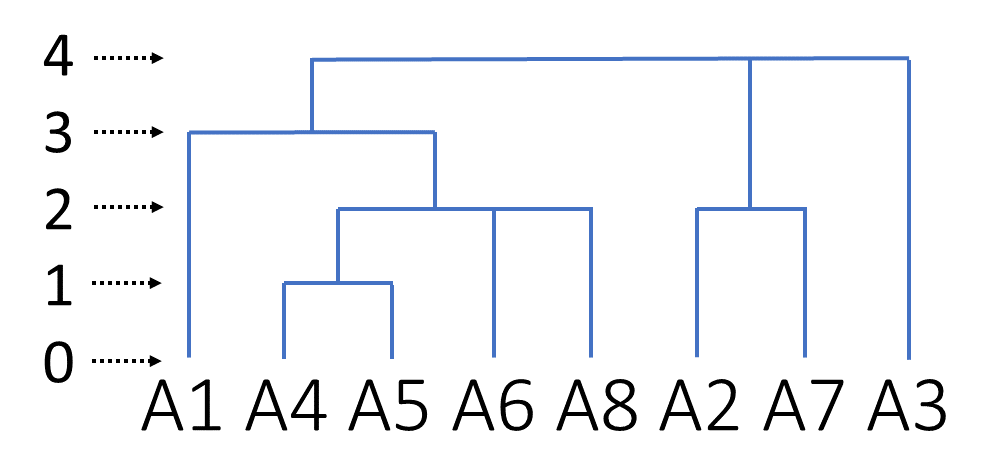
\includegraphics[width=0.45\textwidth]{../imgs/dendrogram.png}
    \end{figure}
\end{frame}

%-------------------------------------------------------------------------------
\begin{frame}
    \frametitle{DBSCAN: Density-based Clustering}
    
    \begin{itemize}
        \item DBSCAN: Density-Based Spatial Clustering of Applications with Noise
        \item \textbf{Density:} The number of points within a specified radius ($\epsilon$)
        \item \textbf{MinPts (min\_samples):} A point is a \textbf{core point} if it has at least \textbf{MinPts} within $\epsilon$.
        \item A \textbf{border point} is not a \textbf{core point}, but is in the neighborhood of a core point.
        \item A \textbf{noise point} is any point that is not a core point or a border point.
    \end{itemize}

    Limitations:
    \begin{itemize}
        \item Clusters with varied densities
        \item High dimensional data
    \end{itemize}
    
\end{frame}

%-------------------------------------------------------------------------------
\begin{frame}
    \frametitle{DBSCAN Pseudocode}
    % \small
    
    % \hrulefill \par
    \begin{figure}
        \centering
        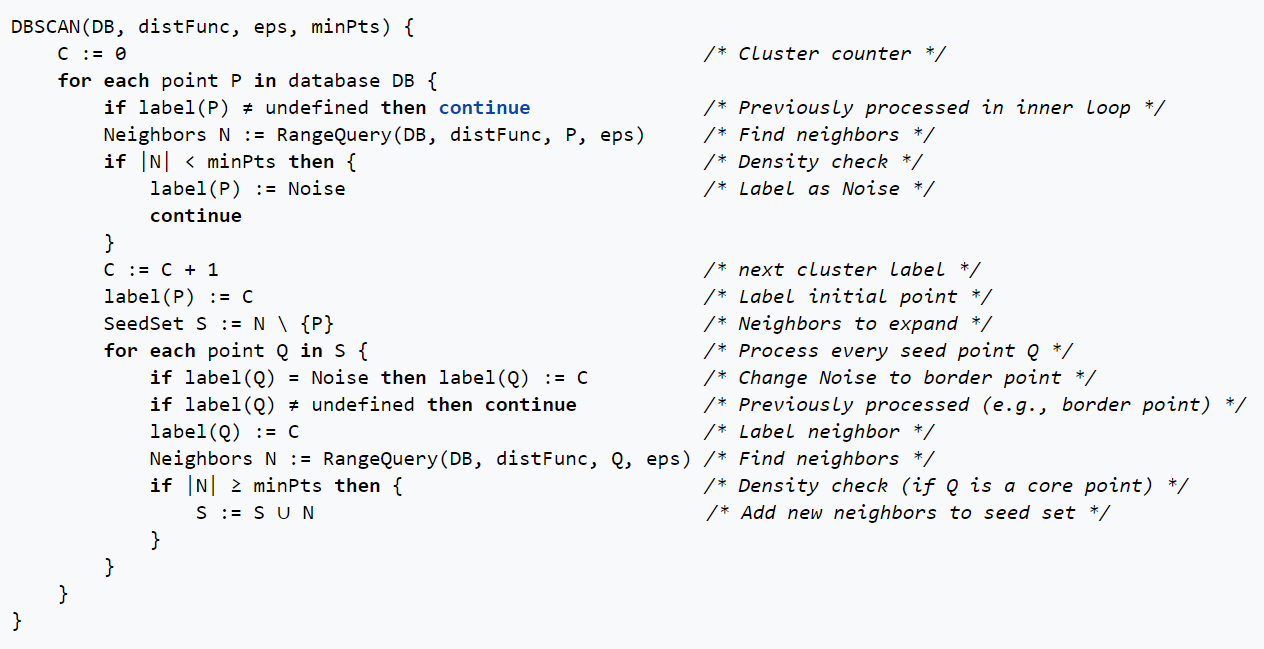
\includegraphics[width=0.9\textwidth]{../imgs/dbscan.png}
    \end{figure}
    % \hrulefill \par
    
\end{frame}


% %-------------------------------------------------------------------------------
% \begin{frame}
%     \frametitle{DBSCAN Pseudocode}
%     % \small
    
%     \hrulefill \par
%     \begin{tabbing}
%         \texttt{DBSC}\=\texttt{AN}($\epsilon$, \textit{MinPts}):\\
%         \> $C := 0$\hspace{2em}\# Current number of cluster\\
%         \> \textbf{For} \= each unvisited point $p$:\\
%         \> \> Mark $p$ as visited\\
%         \> \> \textit{NeighborPts} $:=$ the neighbours of $p$ within $\epsilon$\\
%         \> \> \textbf{If} \texttt{s}\=\texttt{ize}(\textit{NeighborPts}) < \textit{MinPts}:\\
%         \> \> \> Mark $p$ as \textit{NOISE}\\
%         \> \> \textbf{else}:\\
%         \> \> \> $C := C + 1$\\
%         \> \> \> \texttt{ExpandCluster}($p$, \textit{NeighborPts}, C, $\epsilon$, \textit{MinPts})\\
%     \end{tabbing}
%     \hrulefill \par
    
% \end{frame}

% %-------------------------------------------------------------------------------
% \begin{frame}
%     \frametitle{DBSCAN Pseudocode}
%     % \small
    
%     \hrulefill \par
%     \begin{tabbing}
%         \texttt{Expa}\=\texttt{ndCluster}($p$, \textit{NeighborPts}, C, $\epsilon$, \textit{MinPts})\\
%         \> Add $p$ to cluster $C$\\
%         \> \textbf{For} \=each point $j$ in \textit{NeighborPts}:\\
%         \> \> \textbf{If} $j$ \=is not visited:\\
%         \> \> \> Mark $j$ as visited\\
%         \> \> \> $\textit{NeighborPts}_j :=$ the neighbours of $j$ within $\epsilon$\\
%         \> \> \> \textbf{If} \texttt{s}\=\texttt{ize}(\textit{NeighborPts$_j$}) $\geq$ \textit{MinPts}:\\
%         \> \> \> \> $\textit{NeighborPts} := \textit{NeighborPts} \cup \textit{NeighborPts}_j$\\
%         \> \> \> \textbf{If} $j$ is not yet a member of any cluster:\\
%         \> \> \> \> add $j$ to cluster $C$\\
%     \end{tabbing}
%     \hrulefill \par
    
% \end{frame}

%-------------------------------------------------------------------------------
\begin{frame}
    \frametitle{Cluster Cohesion and Separation}
    
    \textbf{Cluster Cohesion}
    \begin{itemize}
        \item Measures how closely related are data points in a cluster
        \item \textit{Within Cluster Sum of Squares} (WCSS) = \textit{Sum of Squared Error} (SSE)
    \end{itemize}

    \[
        \text{SSE} = \sum^{K}_{i=1} \sum_{x \in C_i} ||x - m_i||^2
    \]

    % \vspace{1em}
    \textbf{Cluster Separation}
    \begin{itemize}
        \item Measure how distinct or well-separated a cluster is from other clusters
        \item \textit{Between cluster Sum of Squares} (BSS) a.k.a. \textit{Sum of Squared Between} (SSB)
    \end{itemize}

    \[
        \text{SSB} = \sum^{K}_{i=1} |C_i|(m - m_i)^2
    \]

    where $|C_i|$ is the size of cluster $i$, $m$ is the grand mean, $m_i$ is the mean for the cluster $i$.
    
\end{frame}

%-------------------------------------------------------------------------------
\begin{frame}
    \frametitle{Cluster Cohesion and Separation}

    \begin{itemize}
        \item \textit{Sum of Squares Total} (SST): The sum of squares between the n data points and the grand mean
    \end{itemize}

    \[
        \text{SST} = \text{SSB} + \text{SSE}
    \]

    \begin{itemize}
        \item SST is a constant based on the observed data points. 
        \item The same terminologies are used in the one-way analysis of variance (\textbf{ANOVA}) test.
    \end{itemize}
        
\end{frame}

%-------------------------------------------------------------------------------
\begin{frame}
    \frametitle{Sums of Squares (SS) Example}

    \begin{example}
        Divide 1D data points $\{1,2,3,6,7\}$ into 2 clusters: $\{1,2,3\}$ and $\{6,7\}$. 
    \end{example}
    
    \begin{itemize}
        \item $n = 5$, $|C_1|=3$, and $|C_2|=2$
        \item $m = (1 + 2 + 3 + 6 + 7)/5 = 3.8$
        \item $m_1 = (1 + 2 + 3)/3=2$
        \item $m_2 = (6+7)/2=6.5$
    \end{itemize}

    \begin{equation*}
        \begin{array} {rl}
            \text{SSB} & = 3(3.8-2)^2 + 2(3.8-6.5)^2 = 24.3 \\
            \text{SSE} & = (1-2)^2 + (2-2)^2 + (3-2)^2 + (6-6.5)^2 + (7-6.5)^2 = 2.5 \\
            \text{SST} & = \text{SSB} + \text{SSE} = 24.3 + 2.5 = 26.8 \\
        \end{array}
    \end{equation*}

    The alternative way to compute SST:
    \begin{equation*}
        \begin{array} {rl}
            \text{SST} & = (1-3.8)^2 + (2-3.8)^2 + (3-3.8)^2 + (6-3.8)^2 + (7-3.8)^2 = 26.8
        \end{array}
    \end{equation*}
    
\end{frame}

%-------------------------------------------------------------------------------
\begin{frame}
    \frametitle{Silhouette Coefficient}
    \small

    \textbf{Silhouette coefficient} combines ideas of both cohesion and separation, but for individual points.
    
    For each data point, $i$:\\
    \textbf{a:} The mean distance between a sample and all other points in the same class
    \begin{equation*}
        a(i) = \frac{1}{|C_i|-1} \sum_{j \in C_i, y \neq i}d(i, j)
    \end{equation*}
    \textbf{b:} The mean distance between a sample and all other points in the \textbf{next nearest cluster}
    \begin{equation*}
        b(i) = \min_{k \neq i} \frac{1}{|C_k|} \sum_{j \in C_k}d(i, j)
    \end{equation*}
    
\end{frame}

%-------------------------------------------------------------------------------
\begin{frame}
    \frametitle{Silhouette Coefficient for the Entire Dataset}
    
    The Silhouette Coefficient for a single sample $s(i)$ is then given as:
    \begin{equation*}
        s(i) = 
        \begin{cases}
            1 - a(i) / b(i) & \text{, if }a(i) < b(i)\\
            b(i) / a(i) - 1 & \text{, if }a(i) \leq b(i)
        \end{cases}
    \end{equation*}

    \begin{itemize}
        \item The Silhouette Coefficient for a set of samples is given as the mean of the Silhouette Coefficient for each sample.
        \item The range is in $[0, 1]$, the \textbf{larger} the better.
    \end{itemize}
    
    \begin{example}
        \href{https://scikit-learn.org/stable/auto_examples/cluster/plot_kmeans_silhouette_analysis.html}{An example from \textit{sklearn}}
    \end{example}
\end{frame}

%-------------------------------------------------------------------------------
\begin{frame}
    \frametitle{Overview of Clustering Methods From \textit{sklearn}}
    
    \begin{example}
        \href{https://scikit-learn.org/stable/modules/clustering.html}{The \textit{sklearn} Documentation for Clustering}
    \end{example}
    
\end{frame}

\end{document}


